\documentclass[oneside,a4paper]{book}
%\pagestyle{headings}


%=============================================================================
\usepackage{amsthm}
\usepackage{xspace}
\usepackage{float}
\usepackage{ifthen}
\usepackage{amsbsy}
\usepackage{amssymb}
\usepackage{balance}
\usepackage{booktabs}
\usepackage{graphicx}
\usepackage{rotating}
\usepackage{multirow}
\usepackage{needspace}
\usepackage{microtype}
\usepackage{bold-extra}
\usepackage{geometry}
\usepackage{varioref}
\usepackage{xcolor}
\usepackage{textcomp}
\usepackage{listings}
\usepackage[normalem]{ulem} %emphasize still italic
\usepackage{ucs}
\usepackage{mathtools}
\usepackage{booktabs}
\usepackage{colortbl}
\usepackage{longtable}
% \usepackage[utf8]{inputenc}
% \usepackage[htt]{hyphenat}
\usepackage{times}
\usepackage{url}
\usepackage{alltt}
\usepackage{amsmath}
\usepackage{xfrac}
\usepackage{subfigure}
\usepackage{appendix}
\usepackage{stmaryrd}   % for the \shortuparrow
\usepackage[utopia]{quotchap}
\usepackage{pifont}

\usepackage{setspace}
\usepackage[numbers, sort&compress]{natbib}
\usepackage{mdwlist} 
\usepackage{pgfplots}           % Zum erstellen von mathematischen Diagrammen, wie Balken, Flächen usw. 
\usepackage{pgfplotstable}
\definecolor{blueaccent}{RGB}{0,150,214}
\definecolor{darkgray}{RGB}{135,137,139}
\definecolor{mediumgray}{RGB}{185,184,187}
\definecolor{lightgray}{RGB}{202,200,204}
\definecolor{white}{RGB}{255,255,255}
       % support for better spaced lists
% allows for temporary adjustment of side margins
\usepackage{chngpage}
\usepackage[normalem]{ulem} 

\lstset{
	backgroundcolor=\color{lbcolor},
	tabsize=4,
	rulecolor=,
	language=C++,
        basicstyle=\scriptsize,
        upquote=true,
        aboveskip={1.5\baselineskip},
        columns=fixed,
        showstringspaces=false,
        extendedchars=true,
        breaklines=true,
        prebreak = \raisebox{0ex}[0ex][0ex]{\ensuremath{\hookleftarrow}},
        frame=single,
        showtabs=false,
        showspaces=false,
        showstringspaces=false,
        identifierstyle=\ttfamily,
        keywordstyle=\color[rgb]{0,0,1},
        commentstyle=\color[rgb]{0.133,0.545,0.133},
        stringstyle=\color[rgb]{0.627,0.126,0.941},
}
% constants

\newcounter{qcounter}

% commands
\newcommand{\n}{$\cdot$}
\newcommand{\y}{\checkmark}
\newcommand{\subscript}[1]{$_{\textrm{\footnotesize{#1}}}$}
\newcommand{\superscript}[1]{$^{\textrm{\footnotesize{#1}}}$}
\newcommand{\vertical}[1]{\raisebox{-4em}{\begin{sideways}{#1}\end{sideways}}}

\newboolean{showedits}
\setboolean{showedits}{true} % toggle to show or hide edits
\ifthenelse{\boolean{showedits}}
{
       \newcommand{\ugh}[1]{\textcolor{red}{\uwave{#1}}} % please rephrase
       \newcommand{\ins}[1]{\textcolor{blue}{\uline{#1}}} % please insert
       \newcommand{\del}[1]{\textcolor{red}{\sout{#1}}} % please delete
       \newcommand{\chg}[2]{\textcolor{red}{\sout{#1}}{\ra}\textcolor{blue}{\uline{#2}}} % please change
}{
       \newcommand{\ugh}[1]{#1} % please rephrase
       \newcommand{\ins}[1]{#1} % please insert
       \newcommand{\del}[1]{} % please delete
       \newcommand{\chg}[2]{#2}
}


% ============================================================================
% Put edit comments in a really ugly standout display

\usepackage{xcolor}
\usepackage[normalem]{ulem}
\newcommand{\ra}{$\rightarrow$}


% comments \nb{label}{color}{text}
\newboolean{showcomments}
\setboolean{showcomments}{true}
\ifthenelse{\boolean{showcomments}}
    {\newcommand{\nb}[3]{
        {\colorbox{#2}{\bfseries\sffamily\scriptsize\textcolor{white}{#1}}}
        {\textcolor{#2}{\sf\small$\blacktriangleright$\textit{#3}$\blacktriangleleft$}}}
     \newcommand{\version}{\emph{\scriptsize$-$Id$-$}}
%	 \newcommand{\ugh}[1]{\textcolor{red}{\uwave{#1}}} % please rephrase
%	 \newcommand{\ins}[1]{\textcolor{blue}{\uline{#1}}} % please insert
%	 \newcommand{\del}[1]{\textcolor{red}{\sout{#1}}} % please delete
%	 \newcommand{\chg}[2]{\textcolor{red}{\sout{#1}}{\ra}\textcolor{blue}{\uline{#2}}} % please change
	 \newcommand{\chk}[1]{\textcolor{ForestGreen}{#1}} % changed, please check
	}
    {\newcommand{\nb}[3]{}
     \newcommand{\version}{}
	\newcommand{\chk}[1]{} % changed, please check
	}

\pgfplotstableread[col sep=comma]{
File-Size, Non-Secured, Secured
64, 2.0358, 2.0413
128, 2.041, 2.04455
256, 2.04985, 2.05925
512,2.0681, 2.07195
1024, 2.0997, 2.1062
}\mytableonenode

\pgfplotstableread[col sep=comma]{
File-Size, Non-Secured, Secured
64, 2.03665, 2.04735
128, 2.04145, 2.04955
256, 2.04995, 2.06065
512, 2.073, 2.07325
1024, 2.10175, 2.1093
}\mytabletwonodes

\pgfplotstableread[col sep=comma]{
File-Size, Non-Secured, Secured
64, 2.0383, 2.05
128, 2.0437, 2.0502
256, 2.0507, 2.06565
512, 2.07045, 2.0766
1024, 2.10955, 2.11625
}\mytablethreenodes

% ============================================================================
% Make quotes be italic
\renewenvironment{quote}
    {\list{}{\rightmargin\leftmargin}%
     \item\relax\begin{it}}
    {\end{it}\endlist}

\newcommand{\ttimes}{\ensuremath{\times}}

%=============================================================================

\newcommand{\needlines}[1]{\Needspace{#1\baselineskip}}

% source code
\usepackage{xcolor}
\usepackage{textcomp}
\usepackage{listings}
\definecolor{source}{gray}{0.9}
\lstset{
	language={},
	% characters
	tabsize=3,
	upquote=true,
	escapechar={!},
	keepspaces=true,
	breaklines=false,
	alsoletter={:},
	breakautoindent=true,
	columns=fullflexible,
	showstringspaces=false,
	basicstyle=\footnotesize\ttfamily,
	% background
	frame=single,
    framerule=0pt,
	backgroundcolor=\color{source},
	% numbering
	numbersep=5pt,
	numberstyle=\tiny,
	numberfirstline=true,
	% captioning
	captionpos=b,
	numberbychapter=false,
	% formatting (html)
	moredelim=[is][\textbf]{<b>}{</b>},
	moredelim=[is][\textit]{<i>}{</i>},
	moredelim=[is][\uline]{<u>}{</u>}}
\newcommand{\ct}{\lstinline[backgroundcolor=\color{white},basicstyle=\footnotesize\ttfamily]}
\newcommand{\lct}[1]{{\small\tt #1}}


%----------------------------------------------------------------------------
% references
\newcommand{\tabref}[1]{\hyperref[{tab:#1}]{Table~\ref*{tab:#1}}}
\newcommand{\figref}[1]{\hyperref[{fig:#1}]{Figure~\ref*{fig:#1}}}
\newcommand{\secref}[1]{\hyperref[{sec:#1}]{Section~\ref*{sec:#1}}}
\newcommand{\lstref}[1]{\hyperref[{lst:#1}]{Listing~\ref*{lst:#1}}}
\newcommand{\charef}[1]{\hyperref[{cha:#1}]{Chapter~\ref*{cha:#1}}}
%----------------------------------------------------------------------------

% abbreviations
\tracingcolors 4
\setcounter{tocdepth}{3}
\setcounter{secnumdepth}{3}
\newcommand{\ie}{\emph{i.e.,}\xspace}
\newcommand{\eg}{\emph{e.g.,}\xspace}
\newcommand{\etc}{\emph{etc.}\xspace}
\newcommand{\etal}{\emph{et al.}\xspace}


\newcommand{\newevenside}{
	\ifthenelse{\isodd{\thepage}}{\newpage}{
	\newpage
        \phantom{placeholder} % doesn't appear on page
	\thispagestyle{empty} % if want no header/footer
	\newpage
	}
}

\def\stretchfactor{1}
\newcommand{\mychapter}[1]{\setstretch{1}
    \chapter{#1}\setstretch{\stretchfactor}}

%----------------------------------------------------------------------------
\newcommand{\lessSpace}{\vspace{-1em}}
\DeclareGraphicsExtensions{.pdf,.png}
\graphicspath{{images/}}
\newcommand{\fig}[4]{
	\begin{figure}[#1]
		\centering
		\includegraphics[width=#2\textwidth]{#3}
		\lessSpace
		\caption{\label{fig:#3}#4}
	\end{figure}}

% ===========================================================================


\newcommand{\thesistitle}{A Practice Approach to Proof of Data Possession with Merkle Hash Trees}
\newcommand{\thesisauthor}{Anukriti Shrimal}
\newcommand{\thesisleiter}{Dr. Pascal Felber, Complex Systems, Faculté des sciences, Université de Neuchâtel, Supervisor}
\newcommand{\thesisasst}{Dr. Valerio Schavioni, Complex Systems, Faculté des sciences, Université de Neuchâtel, Supervisor}
\newcommand{\thesissubtitle}{}
\newcommand{\thesisdate}{\today}



% ===========================================================================

\usepackage[ colorlinks=true, urlcolor=blue, linkcolor=black,
			citecolor=black, bookmarksnumbered=true, bookmarks=true,
			plainpages=false,
			pdftitle={\thesistitle}, pdfauthor={\thesisauthor},
			pdfsubject={\thesissubtitle}, pdfpagelabels]{hyperref}

\newcommand{\hrref}[2]{\hyperref}
% ===========================================================================
% ===========================================================================


% D O C U M E N T
% % % % % % % % % % % % % % % % % % % % % % % % % % % % % % % % % %
\begin{document}

% T I T L E
% % % % % % % % % % % % % % % % % % % % % % % % % % % % % % % % % %
\begin{titlepage}  
  \begin{center}  
  
  \begin{figure}[t]  
  \vspace*{-2cm}        % to move header logo at the top 
  \center{
\includegraphics[scale=0.2]{MSc_quer}}
  \vspace{0.4in}     
  \end{figure}

    \thispagestyle{empty}
    
    {\bfseries\Huge \thesistitle \par
    \Large \vspace{0.1in} \thesissubtitle \par}

    \vspace{0.3in} 
    \LARGE{\textbf{Master Thesis} \\}
    \vspace{0.4in}

    {\Large \thesisauthor}
    
    \vspace{0.3in}
    {\Large \thesisleiter}
    
    \vspace{0.3in}
    {\Large \thesisasst}
    
    \vspace{0.3in}
    {\Large Home University \par}
    {\Large Universit\"{a}t Bern \par}
    \vfill
    {\Large \thesisdate \par}
  

  \vspace{0.9in}
 
  % === Logos ==============================================     
  \begin{figure}[htp]
    \centering
    
\includegraphics[scale=0.30]{UNI_Bern.png}\hfill
    
\includegraphics[scale=0.30]{UNI_Neuenburg.png}\hfill
    
\includegraphics[scale=0.80]{UNI_Fribourg.png}
  \end{figure}
  % === // Logos ===========================================    


  \end{center}

\end{titlepage}

\chapter*{\centering Acknowledgement}
I would like to sincerely thank my guide Prof. Dr. Pascal Felber for offering me the chance to research and implement such a challenging and exciting topic for my Master’s thesis. I also wish to express my immense gratitude to my supervisor Dr. Valerio Schavioni who made it possible for me to complete this work. During the entire duration of the project, he provided me with continuous motivation, resources to guide me in my research and constant feedback to make improvements in work. 


On the personal front, I would like to thank my son Ayaan, who was born in the midst of project duration, who inspired me to finish this work. I am also indebted to my family and work colleagues who provided my with support whenever I needed. Finally, I would like to dedicate this thesis to my husband, Prakash who provided me with support and motivation and without whom this could not have been possible.

% A B S T R A C T
% % % % % % % % % % % % % % % % % % % % % % % % % % % % % % % % % %
\chapter*{\centering Abstract}
\begin{quotation}
\noindent 
With Infrastructure as a Service (Iaas) and Software as a Service(SaaS), cloud is one of the most popular storage alternatives today providing low cost solutions. Cloud providers currently do not provide any security mechanisms to assure users of their data possession, as such mechanisms are generally computation, network and/or storage heavy. This is one of the reasons why public cloud providers are not trusted as reported by several studies.\cite{MCAFEE}\cite{FDS}. 

This thesis aims at studying the various approaches that can be employed to solve this problem. It then goes on to choose one such scheme using Merkle hash Tree and Radix Path Identifier based on its merits over other options.
The thesis later proposes a concrete algorithm and implements a proof of concept to provide Proof of Data Possession which is low in network and storage overhead, while being reliable and secure. It then concludes with the evaluation the performance of the algorithm and discusses future work.

The proof of concept and test results for the proposed algorithm can be found at \href{https://github.com/anushrimal/PDP_Master_Thesis.git}{PoDP Implementation}.  
 
 

\end{quotation}
\clearpage

% C O N T E N T S 
% % % % % % % % % % % % % % % % % % % % % % % % % % % % % % % % % % % % % % % %
\tableofcontents

%%%%%%%%%%%%%%%%%%%%%%%%%%%%%%%%%%
%%%% NEW CHAPTER %%%%%%%%%%%%%%%%%%%%%
%%%%%%%%%%%%%%%%%%%%%%%%%%%%%%%%%%
\chapter{Introduction}
\label{cha:introduction}
In this age of digitalization and smart devices, cloud platforms have emerged as the primary storage alternatives because they offer advantages like high availability, convenience of storage, almost zero maintenance, replication, ease of use and synchronization at very low costs. Major public cloud players like Amazon, Google and Dropbox provide such solutions at costs as low as CHF 2/month. Despite of all the advantages, one area where all cloud storage solutions under-perform is security. Commonly known security threats include data loss and data breach resulting from hardware or software failure, human error and targeted attacks. As reported in the recent survey by McAffe\cite{MCAFEE}, 1 in 4 organizations who use Infrastructure-as-a-Service (IaaS) or Software-as-a-Service (SaaS) have had data stolen, and 1 in 5 have experienced an advanced attack against their public cloud infrastructure. \paragraph{} 

One of the biggest concerns among users is permanently losing their data because news reports of data loss by different providers are not rare. Though the percentage of permanent data losses in reported incidents by many providers like Google\cite{bbc}, Dropbox\cite{dropbox}, U.S. Healthcare\cite{Hitrust}, etc. is quite low, it has resulted in decreased trust in the storage solutions. Most cloud providers have done nothing to alleviate these issues, leading to distrust in the cloud-platforms themselves. 
    
This is because once the user outsources some data, he/she loses physical access and management control over the infrastructure holding the data. As cloud providers lack transparency and have no mechanisms to ensure their customers about fresh, correct, complete data possession. The cloud-provider might store the data once and never record any updates to it by user. They can delete parts of data like compress image and store it. The users have no way to determine if their outsourced data is correctly stored by the provider without actually retrieving the data and then comparing it with a local copy.  This, in turn, defeats the purpose of outsourcing data in the first place. In most cases, the data is outsourced to reduce local storage requirements, thus making this security check impossible. 
\paragraph{}


So it is quite critical for cloud platforms to provide a mechanism that enables the user to ensure data possession and integrity. The ability of a storage system to generate proofs of possession of the client's data, without having to
retrieve the whole file, is called Proof of Data Possession (PoDP) ~\cite{PDPDef}.\paragraph{}

This paper provides a Proof of Data Possession algorithm with its implementation details, Proof of Concept and its performance impact. The overall goal of this algorithm is to ensure data integrity to data owners by cloud/storage provider with very little overhead in terms of network bandwidth, computation, and storage. The Proof of Concept and test results for the proposed algorithm can be found on GitHub as git repository named \href{https://github.com/anushrimal/PDP_Master_Thesis.git}{PoDP Implementation}.

\chapter{Problem Statement}
\label{cha:Problem Statement}
When a user wants to store his/her data on a cloud platform, the following entities come into play:
\begin{itemize}
\item The client application, found on the user's device. This client application is responsible to send data to the cloud using a predefined protocol.
\item The remote server, which determines where user's data should be sent based on replication count. Public storage cloud-providers (like Amazon EFS, Dropbox etc.) keep more that one copy/replica of stored data in more than one geographical location. 
\item Cluster node (as selected by the server), the device responsible for storage and later retrieval of data.
\end{itemize}
Once the user stores the data on cloud, in many cases he/she deletes the local copy of the data. It is now assumed that the cloud provider safely stores the data in one or more of its cluster nodes. The cloud provider might, however, lose the data in the following scenarios:
\begin{enumerate}
\item Unintentionally, due to software/hardware failure. In this case, the cloud provider might skip informing the user about the loss of data.
\item Intentionally. All cluster nodes have their users' data storage and retrieval statistics. This means that they are aware of the data, never or most rarely retrieved by the user. So in order to free-up space, they might overwrite any old, seemingly less important data. 
\end{enumerate}
In both cases, the user remains unaware of data loss until he/she tries to retrieve the data and the cloud provider is unable to do so. Or the provider might return some invalid data, but the user does not have anything to compare it with for validity.
It is because of this unaccountability of cloud providers, there needs to be a mechanism in place which ensures that the cloud provider is still in possession of the data, with a limited amount of time and computational overheads. 
\chapter{Related Work}
\label{cha:Related Work}
Much research work is being done to solve the accountability problem as mentioned in previous section. Juels and Kaliski were the first to introduce an efficient audit protocol through which a server could prove data retrievability ~\cite{JnK}. Their POR protocol encrypts the file and randomly embeds a set of randomly-valued check blocks or error-correcting codes called sentinels. One important drawback of this algorithm is that it involves the modification of user-data before storage. Also, if error-correcting codes are used as sentinels, it increases computational overhead and storage overhead (around 15\%). \paragraph{} 

Yevgeniy Dodis, Salil Vadhan, and Daniel Wichs formally defined Proof of Retrievability (PoR) codes for the first time in terms of a triple of functions (Init, Read, Resp).   ~\cite{PoRHardness}. They discussed the probability of attacks and complexity for each possible technique. \paragraph{} 

Décio Luiz Gazzoni Filho and Paulo Sérgio Licciardi Messeder Barreto\cite{DPS} also provide an algorithm using RSA hashing algorithm in case of peer to peer distributed systems. They also introduced the idea of using a central server to keep track of hashes for each piece of data in the network. However, since the technique depends on a single hash value per file, it has limitations. When there are multiple colluding replicas, only one of them can retain the hash value and share it with others. Also, it cannot be used multiple times. \paragraph{}

Shuai Han, Shengli Liu, Kefei Chen and Dawu Gu provide a Proof of Data Possession (PoDP) algorithm using Maximum Rank Distance (MRD) \cite{PDPDef}. The client file is encoded block-wise to generate homomorphic tags with the help of an MRD code. In an audit, the storage provider is able to aggregate the blocks and tags into one block and one tag, due to the homomorphic property of tags. \paragraph{} 

Muhammad Saqib Niaz and Gunter Saake have taken forward the concept of homomorphic tags using Merkle hash trees. They suggest dividing the file into blocks and generating hashes for each block. Further, the block hashes are combined to generate a Merkle hash tree. This technique has the advantage of reusability, lower network, and storage overhead. However, it has a high computational overhead in client application which could be a limitation, especially for users with less powerful devices.  ~\cite{Paper13}. \paragraph{}

All these algorithms try to take the concept of data possession/retrieval further. Some of these techniques have a disadvantage of storage of large amounts of data by the client, while others have a large computational overhead.  \paragraph{}

In this paper, we propose an algorithm that takes the concept from the aforementioned algorithms combining the advantages of them. We also implemented the algorithm to study the performance impact of the solution, thus proving it to be a more efficient way to solve the problem of PoDP.
The algorithm takes forward the case where PoDP is provided using a Merkle hash tree and storing them using the Radix path identifiers, which have been explained in detail in the next chapter. The table below explains 3.1 details the differences in each of the approaches.
\begin{table}[]
\centering
\caption{Comparison between various proof of retrievability algorithms}
\label{tab:comparisonTab}
\resizebox{\textwidth}{!}{%
\begin{tabular}{|l|l|c|c|c|c|}
\hline
\rowcolor{mediumgray} 
\textbf{S.No.} & \textbf{Algorithm}                                                     & \multicolumn{1}{l|}{\cellcolor{mediumgray}\textbf{File-modification}} & \multicolumn{1}{l|}{\cellcolor{mediumgray}\textbf{Re-usability}} & \multicolumn{1}{l|}{\cellcolor{mediumgray}\textbf{Resonable overhead}} & \multicolumn{1}{l|}{\cellcolor{mediumgray}\textbf{Central-Server}} \\ \hline
1              & Juels and Kaliski                                                      & \ding{51}                                              & \ding{51}                                         & \ding{55}                                               & \ding{55}                                           \\ \hline
2              & D´ecio Luiz Gazzoni Filho and Paulo S´ergio Licciardi Messeder Barreto & \ding{55}                                              & \ding{55}                                         & \ding{51}                                               & \ding{51}                                           \\ \hline
3              & Shuai Han, Shengli Liu, Kefei Chen and Dawu Gu                         & \ding{51}                                              & \ding{55}                                         & \ding{55}                                               & \ding{55}                                           \\ \hline
4              & Muhammad Saqib Niaz and Gunter Saake                                   & \ding{55}                                              & \ding{51}                                         & \ding{51}                                               & \ding{55}                                           \\ \hline
5              & Proposed algorithm with Merkle hash tree and trusted central-server    & \ding{55}                                              & \ding{51}                                         & \ding{51}                                               & \ding{51}                                           \\ \hline
\end{tabular}}
\end{table}
\chapter{Background}
An important building block of the proposed algorithm is the  Merkle hash tree which is stored in the form of B+ tree and evaluated using Radix Path Identifiers. So to grasp the functioning of the algorithm, it is essential to understand these concepts beforehand. 
\section{Merkle hash tree}
A Merkle hash tree is a tree-based cryptographic data structure in which the hash values/tags of each data block are at the leaves of the tree and every non-leaf node is labelled with the cryptographic hash of the labels of its child nodes.~\cite{MHT} Hash trees have been used in cryptography as they allow efficient and secure verification of file/data contents.
For example, in a simple binary hash tree with two leaves with Hash values(0-0) and (0-1), hash 0 would be the result of hashing the concatenation of hash 0-0 and hash 0-1. That is, hash 0 = hash( hash(0-0) + hash(0-1) ) where + denotes concatenation.

\begin{figure}[h]
\caption{ Merkle hash tree}
\centering
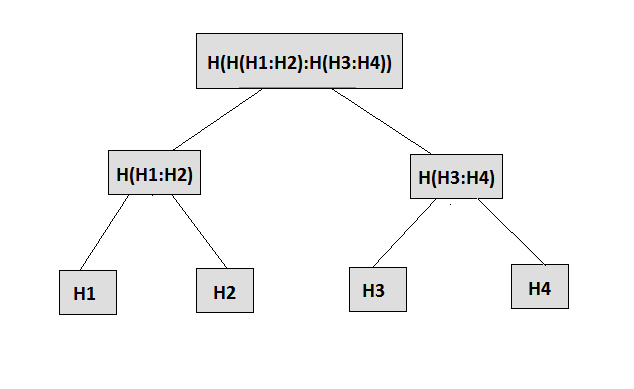
\includegraphics[width=0.8\textwidth]{Merkle_tree}
\end{figure}
    
\section{B+ tree}
A B+ tree is an n-ary tree with a variable but often a large number of children per node. A B+ tree consists of a root, internal nodes, and leaves. The root may be either a leaf or a node with two or more children.

The primary value of a B+ tree is in storing data for efficient retrieval in a block-oriented storage context, making them ideal for our use-case. This is primarily because unlike binary search trees, B+ trees have very high fanout, which reduces the number of I/O operations required to find an element in the tree.

Since Merkle hash tree involves storing file block hashes at leaf node and traversing nodes at different levels to reach the root node, implementing it using a B+ tree seems like an ideal choice in terms of storage and computation. 

So in our algorithm, Merkle hash tree is an n-ary B+ tree structure where each node can hold at most o+1 nodes, where o is the order of the tree.

\section{Radix Path Identifier}
An important requirement of the chosen PoDP scheme is to efficiently store, retrieve and re-evaluate the root hash value of the Merkle hash tree from the leaf hash values on every challenge request by the client. 

To encode, store and later decode and re-evaluate the Merkle hash tree, we have made use of the Radix Path Identifier  as proposed by Muhammad Saqib Niaz and Gunter Saake ~\cite{Paper13} in their paper, and  Vijay Atluri and Günther Pernul ~\cite{IntegrityBook} in their book. 

The basic idea of using Radix Path Identifier(RPI) is to assign a unique number to each node in the Merkle hash B+ tree so that its level can clearly be identified and its parent node can be easily derived. In order to generate this unique number, radix or base value needs to be defined. For our implementation we defined the order of the generated Merkle hash tree (max nodes that can be contained in an internal node) to be used as the radix r\textsubscript{b}. Now if l is the level of a node and i is the index of a value within the node, RPI value of each node can be defined as explained below:      

\[
    rpi = 
\begin{dcases}
    \ l+i, & \text{if}\ l=0 \\
 	\ rpi_{parent} * r_{b} + i, & \text{if}\ l>0
\end{dcases}
\]

In order to better understand how it works, consider Figure 4.2. Assume that the file is divided into 6 blocks - indexed 1 to 6. These blocks are then inserted into the B+ tree of order 3. After all the blocks are inserted, the resultant tree has three levels as shown in the same figure. After the tree is generated, the RPI is generated as per the formula above. For e.g., the root node(l = 0) RPI values will be 0, 1, 2 (= their respective indices). Note that all leaf nodes will always have index 0 and all the calculations done are based on ternary number system. Now consider block 5. As per the formula, its RPI is equal to RPI of its parent multiplied by radix, hence the value 200.

The two important requirements listed above to ensure re-evaluation of the root hash value are fulfilled by this scheme as follows:
\begin{itemize}
\item A node's parent RPI rpi\textsubscript{parent} can be calculated as rpi/r\textsubscript{b}
\item A node pointer's index can also be calculated using formula rpi mod r\textsubscript{b}  
\end{itemize}

\begin{figure}[h]
\caption{ Radix path identifier for Merkle hash tree}
\centering
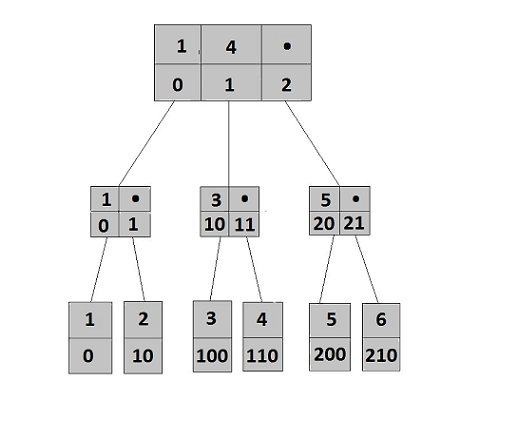
\includegraphics[width=0.8\textwidth]{rpi}
\end{figure}
     
\chapter{Proposed algorithm}
\label{cha:Proposed algorithm}
\section{General approach}
A Proof of Data Possession (PoDP) scheme involves an audit mechanism in which after the storage of his/her data on the cloud, the client can audit the cloud storage at any point of time and get a response with the smallest amount of computation, time and network overhead to ensure that the cloud provider is still in possession of the data.\paragraph{}

Data integrity schemes can be divided into two main categories, i.e., probabilistic and deterministic.
Deterministic techniques ensure complete data possession by the storage system. These techniques are generally storage and computation heavy. 
As the name suggests, probabilistic techniques can only assure that there is a high likelihood of data possession by the storage system. Such schemes generally have lower storage and/or computational overheads, which make them preferred choice of PoDP mechanisms. Also, if probabilistic schemes are used repeatedly over time, they can ensure complete data possession.\paragraph{}

Based on these techniques, the following possible mechanisms can be utilized. Their advantages and drawbacks have also been discussed:
\begin{itemize}
\item A possible solution could be that the client application retains the local copy of the data. The user then requests the entire file data during the challenge/audit phase from the cluster node and then compares the entire file with local file data.
Clearly, this is a deterministic theme which involves high storage overhead, thus defeating the purpose of data outsourcing.
\item Another possible solution could be a probabilistic scheme involving hash function. A hash function is a one-way mathematical function that maps a large-sized data to a smaller fixed-size hash value. Since they are irreversible, i.e., the data cannot be derived from its hash value and they generate a fairly compact code. Hash functions are widely used in multiple PoDP schemes. 

One commonly used scheme is to divide given file data into blocks of fixed size and generate hash values/tags for each block before transmitting the file to the cluster node. During audit, the cluster node is requested to return hash tags for given set of blocks, thus ensuring possession of that many blocks of data.

A problem with this technique is that the block size cannot be kept too large as it reduces the number of times an audit can be performed on the cluster node to ensure data possession. For example, if a file is broken into three blocks, the client can only audit the cluster three times after which, the cluster node could simply store all the hash codes previously requested and delete the file. On any subsequent audit, the cluster node can simply return the stored hash tag, thus making the audits useless. 

If the block size is kept very small, it would result in a large number of tags to be stored at the client's device, thus increasing the storage and network overhead of the algorithm. 

\item Another possible probabilistic technique using hash functions with smaller block sizes involves making use of Merkle hash trees. This technique could also reduce storage and network overhead.

\item In order to reduce the load of computation in the client device, another proposed idea is to make use of a trusted server. It could be a third party server or the remote server within the cloud infrastructure that can bear the burden of computation and storage of Merkle hash tree related information and querying different cluster node replicas on each audit.
The cloud provider could provide this feature to increase trust in its platform. Also, they could embed these qualities in one of their cluster manager/servers.
\end{itemize}

Since the usage of Merkle hash trees using a third-party or cloud remote server seems to be the most optimal solution in terms of computation, network, and storage overhead, we chose this technique to implement it and test its performance.  
\section{Algorithm}
The crux of the algorithm can be divided into three phases - Setup/Init, Challenge and Response. Each of these steps is explained as follows:
\begin{itemize}
\item Setup : Consider a case where a user tries to upload a 32KB file to a cloud by sending the file to a server by cloud-provider. The server upon receiving the file breaks it into blocks of equal sizes applies hash function on each block content and inserts the generated block hashes one by one into an empty B+ tree. The server determines the block size based on the size of the file so that there are a considerable number of blocks. In this case, the server decides the block size to be 8KB, thus resulting in 8 blocks.

Once all block hashes are inserted at leaves into the tree, it needs to traverse it twice. 
\begin{itemize}
\item First, bottom to up combining the hashes until reaching the root. This is shown in Figure 5.1 below.
\begin{figure}[h]
\caption{Merkle b+ hash tree for file with 8 blocks}
\centering
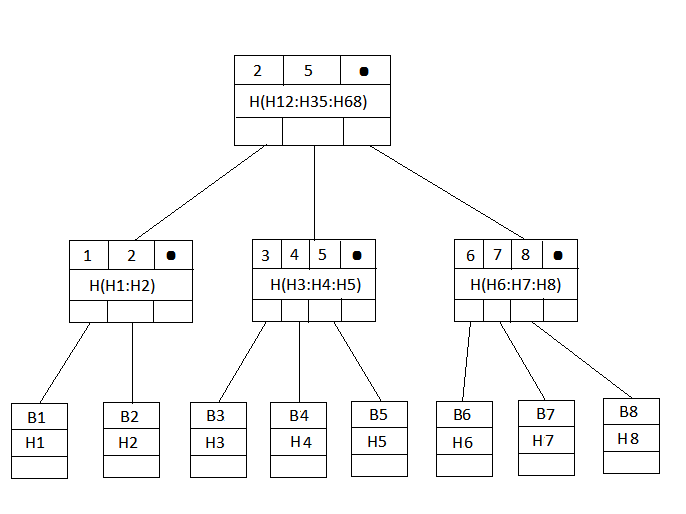
\includegraphics[width=0.7\textwidth]{algo1}
\end{figure} 
\item Secondly, the server traverses it breadth-first starting from the root node, assigning RPI for each value within the node. For example, since the root node contains three values/pointers and it has no parent, its RPI values can be set to 0, 1, 2 respectively for each value. On moving further down to central internal node with parent RPI value 1 and using the RPI generation formula, the RPI for its values/pointers will be 10,11,12 etc. This is shown in Figure 5.2.
\begin{figure}[h]
\caption{RPI indexed B+ hash tree}
\centering
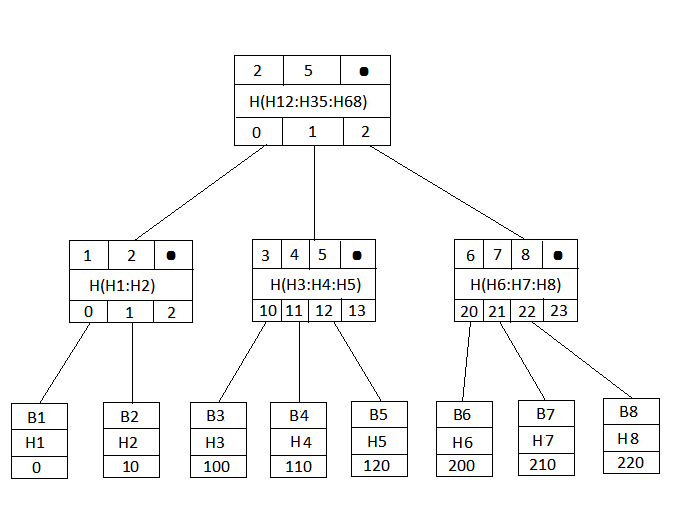
\includegraphics[width=0.7\textwidth]{algo2}
\end{figure}  
\end{itemize}   
The server then stores the generated Merkle hash tree along with the RPI values into its local database as JSON. It also stores the filesize and blocksize of the file. It then forwards the file to cluster nodes and returns the root hash to the user.
\item Challenge : On receiving a challenge for the file, the server selects some blocks randomly which are then queried from one of the cluster nodes. In the current case, assume that the server chooses block numbers 2 and 5 . The cluster node evaluates the hash values and returns them to the server.
\item Response : The server now needs to rebuild the Merkle root hash value using the values returned from the cluster node. The algorithm makes use of RPI to recreate the root hash to use values from the cluster node, when present or its database, otherwise. This is done using a bottom-up depth-first approach. Whenever an internal node has a block which was requested from the cluster, it needs to re-evaluate the node hash value. In the given example, the server retrieves the hash value of block B1 and combines it with hash value returned for B2 from the cluster node to generate H(H1:H2). Similarly, it retrieves the hash values of blocks B3 and B4 to combine them with the value returned for B5 from the cluster node. Since no blocks were requested from previous node, its hash value is simply retrieved from the database. Finally, the newly generated hash values for H12 and H35 are combined with H68 from the database to generate H(H12':H35':H68) and it is returned to the user. The client matches this value with its own stored value to know if one of the replicas indeed stores the file.        
\end{itemize}
   
\section{Architecture}
The exchanges between the client, the remote server and the cluster nodes on the cloud can generally be described as shown in Figure 5.3 below can be explained as follows:
\begin{figure}[h]
\caption{ 	}
\centering
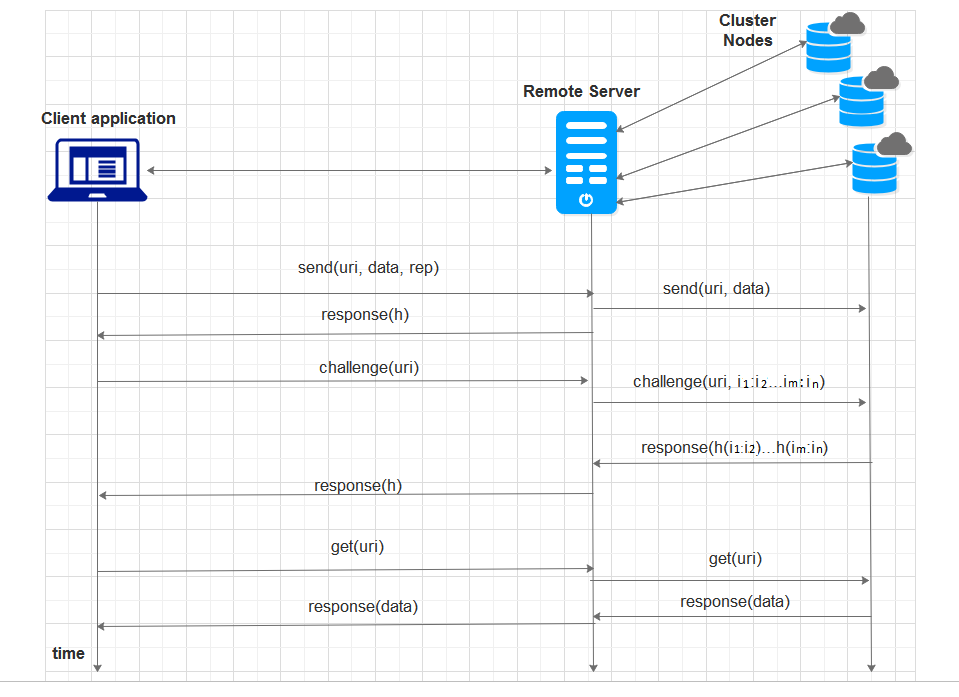
\includegraphics[width=0.8\textwidth]{architecture}
\end{figure}

\begin{enumerate}
\item \emph{send(url, replication count)}\newline
The client application on the user's device sends a local file to be uploaded on the cloud to a remote server.
On receiving the file, the remote server calculates the block size based on file size and generates the Merkle hash tree with hash values of each block. It then sends the file to the required number of cluster nodes based on the replication count. 
On successfully saving the file on each replica, the remote server stores the Merkle hash tree and some metadata  (explained later) in its local database. It then sends the root hash value of the Merkle hash tree to the client application which then stores this root hash in the user's device's local DB.
\item \emph{challenge(file)} \newline
At any later point, the client can query the remote server to generate the proof of data possession by some cluster node. The client can conduct such tests multiple times.

The remote server upon getting this request retrieves the Merkle hash tree and the metadata (like file size, block count, block size) for the file. It then randomly selects one of the cluster nodes and selects around twenty percent of the blocks and sends the list of file indices(i\textsubscript{1}:i\textsubscript{2}...i\textsubscript{m}:i\textsubscript{n}) for which the cluster node should return hashes.
 
\item \emph{challenge(file, i\textsubscript{1}:i\textsubscript{2}...i\textsubscript{m}:i\textsubscript{n})} \newline
The cluster node on receiving this request fetches the file and generates a list of hashes for the indices and returns it as part of response to the remote server.

\item \emph{response(h\textsubscript{12}...h\textsubscript{mn})} \newline
The remote server on receiving the response re-evaluates the Merkle hash tree root value by using the response hashes and hashes of remaining blocks (non-queried) from its local database and sends the response back to the client.

\item \emph{response(h)} \newline
The client on receiving the response verifies it against the hash value stored in its local store to get the PoDP by at least one of the cluster nodes. 

\end{enumerate}
\section{Correctness of Approach}
This section explains why the proposed scheme is secured and optimal in performance. Following are some possible scenarios: 
\begin{itemize}
\item Consider a case where a malicious cluster node deletes the file. Upon receiving a challenge request, it cannot guess the hash values of requested file indexes.
\item Consider a case where a malicious cluster node deletes parts of the file. Since the server can request a hash-value of any random block in the future, there is a good chance of the node getting caught in one of the future challenges.
\item In case there are multiple replicas and all cluster nodes collude, at least one of them will have to retain the file to fulfil future challenge requests.  
\end{itemize}
The possible scenarios where this algorithm might fail are:
\begin{itemize}
\item All block hashes are requested from given replica. In that case, the cluster node can remember the hashes mapped by data indexes and delete the file. This attack is unlikely as the server divides the file in relatively large number of blocks. 
\item A second case where this algorithm might fail is when the server colludes and never forwards a challenge to the cluster node. In order to avoid this, a third-party trusted server can be used. Another alternative is to use SGX, which is explained later in the thesis.
\end{itemize}

\chapter{Implementation details}

The PoC for the proposed Proof of Data possession algorithm is implemented in C++ on Ubuntu platform. It comprises of the following modules, each of which is discussed in detail in further subsections:
\begin{enumerate}
\item A RESTful web server to receive and send files over HTTP.
\item A fast and efficient key-value database to store the Merkle hash tree.
\item Module to split the file into blocks and generate Merkle hash tree(B+ tree) for the file.
\item Module to retrieve and parse the Merkle hash tree and to generate root hash value of the Merkle tree using partial hash values returned from cluster-node and the remaining values from the database.
\end{enumerate}

\section{RESTful Server}
In order to implement the PoC, the first requirement is an appropriate multi-threaded RESTful framework. The framework needs to have a simple implementation for both client and a server providing functionality for standard APIs like POST, GET and custom API that can be extended to implement challenge/Response. Microsoft's cpprestsdk\cite{RestSdk}, Corvusoft's  restbed\cite{Restbed} and Pistache\cite{Pistache} were considered. Corvusoft's restbed was chosen as it has more flexible APIs with a relatively simple implementation. Since the framework is not an inherent part of the algorithm, it can be replaced with any other framework. However, the selected framework needs to provide functionalities described below.

The RestServer is configured to handle GET, POST and CHALLENGE methods and is then started with details about Cluster Nodes.  
\begin{lstlisting}[language=C++]
one->set_method_handler( "POST", postMethodHandler );
two->set_method_handler( "GET", getMethodHandler);
three->set_method_handler( "CHALLENGE", challengeMethodHandler);
\end{lstlisting}

On receiving a POST request, the server downloads the file, generates its Merkle hash tree, stores its encoded version in its local database and then sends the file to cluster-nodes based on replication. To generate the Merkle tree, the server determines the block size and block count  based on file size. It then generates hash values of each block, encodes them and add them to the leaf of the B+ Tree. 
The generated tree is then stored in the local key-value, the file then sent to the cluster node and the root hash value is then  returned to the client
\begin{lstlisting}[language=C++]
int blocksize = getBlockSize(fileData.length());
string rootHash = generateBTree(fileName, fileData, blocksize, order);
session->close( OK, rootHash );
\end{lstlisting}
The generateBTree function has following functionality:   
\begin{lstlisting}[language=C++]
while(remsz > 0) {
	root = btree->insert(root, blocknum, record);
	btree->evaluate(root);
	btree->generate_rpi(root);
	btree->dumpDataOnDB(mDB, filename.c_str(), root, blocksize, blocknum - 1);
}
\end{lstlisting}
On receiving a CHALLENGE request, the server retrieves and decodes the Merkle hash tree in its local database for the requested file. It then selects some random blocks and sends an array of start\_index:end\_index to the cluster node. 

\begin{lstlisting}[language=C++]
rpiA->parse(mDB, body.c_str()/*file URI*/);
int cn_id = rand()%mSendFiles.size();
string response = mSendFiles[cn_id]->challenge(body.c_str(), params);
\end{lstlisting}  

The server then feeds these responses to the algorithm to regenerate the root hash and return it to the client.

\begin{lstlisting}[language=C++]
rpiA->validate(blocknums, hashes, chalRes);
session->close( OK, chalRes, { { "Content-Length", ::to_string( chalRes.size( ) ) } } );
\end{lstlisting} 

In the next section, the generation, encoding, parsing and re-evaluation of the Merkle hash tree is discussed.
\section{Merkle B+ tree}
As explained in sec 6.1, the file is divided into blocks and each block is then inserted into a B+ tree. After all nodes(block hashes) are inserted into the tree, they are at the leaf node of the tree. The block hashes of all children of a node  are concatenated and hashed to make hash value of the parent node. This process is repeated until reaching the root, which then combines the hash value of all the nodes in the tree to generate the tree, a recursive top to bottom approach was used in which block hashes were first added to the root node and then subsequently the nodes are split when they are full. We adapted the B+ tree implementation by Amittai Aviram(which was written in C)\cite{BPlusTree} and modified it to generate Merkle hash values and related metadata and to store it in json format.
    
\section{Radix Path Identifier}
Once the Merkle hash tree has been generated by the server, it needs to store it in its local database until a challenge is received for the file. To do this, RPI is generated for each node of the MHT using a depth-first approach. Thereafter, on receiving a challenge request,  receiving individual block hashes from a cluster node, the remote server loads the hashes of remaining blocks and regenerates the root hash value moving from bottom to top. 
Upon receiving individual block hashes from a cluster node, the remote server loads the hashes of remaining blocks and regenerates the root hash value moving from bottom to top. 
 
\section{Key-value Datastore}
As previously mentioned, the Remote Server needs to store each file's  Merkle hash tree and some metadata. The metadata that is stored per file is required for validation. 
\begin{lstlisting}[language=C++]
proot.put("levels", this->num_level + 1);
proot.put("blockcount", blockcount);
proot.put("blocksize", blocksize);
proot.put("order", this->order);
\end{lstlisting}

The block-hashes with levels and the metadata stated above is encoded in JSON format. It needs to be stored in a key-value store. Redis DB\cite{REDIS} and RocksDB\cite{RocksDB} are two such key-value stores that were considered to store this data. Since RocksDB is an embedded key/value store supporting multi-threaded persistence, it was preferred over Redis DB, which is a remote in-memory store (more suitable when data needs to be stored on another server).
\section{Safety measures}
The safety of this algorithm depends upon the strength of hash function used. We have used openssl's sha256. This is because SHA256\cite{SHA} is currently non-reversible. If one thinks of attacking a SHA256 hash function using brute force, the computation will take more than a lifetime.
\chapter{Analysis and evaluation of the algorithm}
\label{cha:The Performance Evaluation}
Performance impact of a PoDP scheme can be measured in terms of network overhead, storage overhead and computational overhead. Network and storage overhead of this solution is quite low. In terms of storage, the client device only needs to store the file URI and its 256 root hash value. Apart from the file itself, one to four hash values are exchanges between the entities.

The most important performance impact of this algorithm is the computational overhead, thus causing time overhead during POST operation of the file.  
\section{End-to-end tests}
\subsection{Evaluation settings}
In order to account for this time overhead of the implemented PoDP scheme, we tested it on a cluster environment to imitate real life scenarios. It involved following entities:
\begin{itemize}
\item User device with a client application which is simply a shell script with 'curl' commands to send HTTP POST and CHALLENGE requests. We used a Virtual machine to run the client. The tests were performed using files of multiple  sizes ranging from 64KB to 1024KB.
\item Remote server with its own database. The remote server was configured to use one, two or three cluster nodes based on the test-case. We used a physical host to run it.
\item Three cluster nodes each running on a Virtual machine. The count of cluster nodes in each experiment defines the replication count for each file as chosen by client.
\end{itemize}

The tests were performed by taking an average of the time-lags recorded for each operation over two hundred times for different file sizes. The numbers shown in each table and graph is the average value of each scenario of those two hundred runs.
Tests marked secured define the case where the remote server supports our algorithm of generating Merkle hash tree and supporting challenge function calls. Tests marked non-secured are cases where remote-server simple acts as a relay.
\subsection{Results}
As can be seen from Table 7.1, the generation and saving of MHT, RPI and metadata increases the overall response time by 0.01 second on an average irrespective of the file size. This effect can be also be seen in Figure 7.1, 7.2 and 7.3 respectively.  Though it seems like a large overhead for smaller files(64KB), the overhead is still well within reasonable range to enable security and trust in cloud users. Also, the time lag becomes negligible as the size of files increase.

The time overhead of challenge-response APIs was tested as well which is shown in Table 7.2. As expected, the time taken by this API is independent of file-size until files are not extremely large. This is because of the following reasons:
\begin{itemize}
\item On every challenge request, the remote server needs to load and parse RPI based Merkle hash tree and send a single to one of the cluster nodes.
\item On receiving a challenge request, a cluster node needs to load the file from its database and perform hash-functions and return results to the server.
\item In terms of data transmitted, only file URI, indices, hash values, etc. are sent over the network.
\end{itemize} 

  
\begin{table}[]
\centering
\caption{Send file time statistics (in seconds) for secured and non-secured mode}
\label{tab:my-table}
\begin{tabular}{@{}|l|l|l|l|l|l|l|l|@{}}
\toprule
\rowcolor{mediumgray} 
\textbf{S.No.} &
  \textbf{File size (KB)} &
  \multicolumn{2}{l|}{\cellcolor{mediumgray}\textbf{1 Cluster node}} &
  \multicolumn{2}{l|}{\cellcolor{mediumgray}\textbf{2 Cluster nodes}} &
  \multicolumn{2}{l|}{\cellcolor{mediumgray}\textbf{3 Cluster nodes}} \\ \midrule
\multicolumn{2}{|l|}{\textbf{}} &
  \cellcolor{lightgray}\textbf{Non-Secured} &
  \cellcolor{lightgray}\textbf{Secured} &
  \cellcolor{lightgray}\textbf{Non-Secured} &
  \cellcolor{lightgray}\textbf{Secured} &
  \cellcolor{lightgray}\textbf{Non-Secured} &
  \cellcolor{lightgray}\textbf{Secured} \\ \midrule
1 & 64   & 2.0358  & 2.0413  & 2.03665 & 2.04735 & 2.0383  & 2.05    \\ \midrule
2 & 128  & 2.041   & 2.04455 & 2.04145 & 2.04955 & 2.0437  & 2.0502  \\ \midrule
3 & 256  & 2.04985 & 2.05925 & 2.04995 & 2.06065 & 2.0507  & 2.06565 \\ \midrule
4 & 512  & 2.0681  & 2.07195 & 2.073   & 2.07325 & 2.07045 & 2.0766  \\ \midrule
5 & 1024 & 2.0997  & 2.1062  & 2.10175 & 2.1093 & 2.10955 & 2.11625 \\ \bottomrule
\end{tabular}
\end{table}

\begin{table}[]
\centering
\caption{Challenge function time statistics (in seconds)}
\label{tab:tablechallenge}
\begin{tabular}{@{}|l|l|l|l|l|@{}}
\toprule
\rowcolor{mediumgray} 
\textbf{S.No.} & \textbf{File size (KB)} & \textbf{1 Cluster node} & \textbf{2 Cluster nodes} & \textbf{3 Cluster nodes} \\ \midrule
1 & 64   & 0.0272  & 0.0276  & 0.0275  \\ \midrule
2 & 128  & 0.02735 & 0.02735 & 0.02765 \\ \midrule
3 & 256  & 0.0272  & 0.02765 & 0.02755 \\ \midrule
4 & 512  & 0.0269  & 0.02705 & 0.02765 \\ \midrule
5 & 1024 & 0.0273  & 0.02755 & 0.0274  \\ \bottomrule
\end{tabular}
\end{table}

\begin{figure}
\centering
    \begin{tikzpicture}[thick,scale=0.8, every node/.style={scale=0.8}]
      \begin{axis}[
        width=0.8\linewidth,
        ybar=0pt,
        bar width=7.5pt,
        ymin=2.03,
        enlarge x limits={abs=25pt},
        legend style={draw=none,at={(0.5,-0.15)}, text width=2.5cm,
        anchor=north,legend columns=-1},
        xlabel={File size(in KB)},
        ylabel={Time (in seconds)},
        x tick label style={/pgf/number format/1000 sep={}},
        xmajorgrids=true,
        cycle list={blueaccent, mediumgray},
        x tick label as interval,
      ]
        \pgfplotsinvokeforeach{Non-Secured, Secured}{
        \addplot+[draw=none, fill, area legend,] table [col sep=comma,x expr=\thisrow{File-Size}+0.5,y=#1]{\mytableonenode};
        \addlegendentry{#1}
        }
    \end{axis}
    \end{tikzpicture}
    \caption{Performance of secured vs. Non-secured file save on cloud with one cluster node}
    \label{fig:OneNode}
\end{figure}

\begin{figure}
\centering
    \begin{tikzpicture}[thick,scale=0.8, every node/.style={scale=0.8}]
      \begin{axis}[
        width=0.8\linewidth,
        ybar=0pt,
        bar width=7.5pt,
        ymin=2.03,
        enlarge x limits={abs=25pt},
        legend style={draw=none,at={(0.5,-0.15)}, text width=2.5cm,
        anchor=north,legend columns=-1},
        xlabel={File size (in KB)},
        ylabel={Time (in seconds)},
        x tick label style={/pgf/number format/1000 sep={}},
        xmajorgrids=true,
        cycle list={blueaccent, mediumgray},
        x tick label as interval,
      ]
        \pgfplotsinvokeforeach{Non-Secured, Secured}{
        \addplot+[draw=none, fill, area legend,] table [col sep=comma,x expr=\thisrow{File-Size}+0.5,y=#1]{\mytabletwonodes};
        \addlegendentry{#1}
        }
    \end{axis}
    \end{tikzpicture}
    \caption{Performance of secured vs. Non-secured file save on cloud with two cluster nodes}
    \label{fig:OneNode}
\end{figure}

\begin{figure}
\centering
    \begin{tikzpicture}[thick,scale=0.8, every node/.style={scale=0.8}]
      \begin{axis}[
        width=0.8\linewidth,
        ybar=0pt,
        bar width=7.5pt,
        ymin=2.03,
        enlarge x limits={abs=25pt},
        legend style={draw=none,at={(0.5,-0.15)}, text width=2.5cm,
        anchor=north,legend columns=-1},
        xlabel={File size (in KB)},
        ylabel={Time (in seconds)},
        x tick label style={/pgf/number format/1000 sep={}},
        xmajorgrids=true,
        cycle list={blueaccent, mediumgray},
        x tick label as interval,
      ]
        \pgfplotsinvokeforeach{Non-Secured, Secured}{
        \addplot+[draw=none, fill, area legend,] table [col sep=comma,x expr=\thisrow{File-Size}+0.5,y=#1]{\mytablethreenodes};
        \addlegendentry{#1}
        }
    \end{axis}
    \end{tikzpicture}
    \caption{Performance of secured vs. Non-secured file save on cloud with three cluster nodes}
    \label{fig:OneNode}
\end{figure}
\section{Algorithm Performance}
\subsection{Evaluation settings}
The algorithm involves certain variables like block-size and order of the tree, each of which could impact the performance of the algorithm. The order of a tree is defined as the maximum number of values that can be accommodated in a single tree node. As mentioned previously, this algorithm works basically using leaf-nodes and computing up to the root node through intermediate tree-nodes.  

To test the impact of these two variables on the algorithm performance, unit-tests were performed on a single server. This enabled to get pure computation overhead eliminating network overhead. Further details about the tests are as follows:
\begin{itemize}
\item The tests were performed on multiple file-sizes varying from 32KB to 1MB.
\item To test the impact of order, a fixed value of block-size(16KB) was assigned and only order was varied, as seen in Table 8.3.
\item To test the impact of block-size, a fixed value of order(4) was assigned and only block-size was varied, as seen in Table 8.4.
\item Elapsed time was evaluated for the function which breaks the file into blocks, inserts them into the tree, evaluates Merkel hash tree values and dumps it on the DB.
\item Each test was performed 20 times and an average of elapsed-time was then plotted.
\end{itemize}
   
\subsection{Results}
Following observations were can be clearing made from Table 8.3 and 8.4:
\begin{itemize}
\item Computation overhead(in time) keeps decreasing when order or block-size is increased as long as block-count decreases. As block-count decreases, the tree becomes smaller and hence tree traversal and storage time decreases.
\item Computation overhead(in time) remains consistent when increasing or decreasing order/block-size value does not change block-count.
\end{itemize}
It is clear from the above results that both order and block-size play an important role in computation overhead and hence, overall performance of the algorithm. It must however be noted that node-count also defines the number of times the cloud-provider can be challenged. Hence, it cannot be kept too low, as it poses a security threat. 

Hence for our implementation, we kept the order value constant and varied the block-size based on the file-size. An optimum value of block-size is determined from each file to ensure sufficient number of blocks, but also not too high to avoid performance issues. 
\begin{table}[]
\centering
\caption{Effect of order of MHT on algorithm performance (in seconds)}
\label{tab:orderTestFinalTab}
\resizebox{\textwidth}{!}{%
\begin{tabular}{|l|l|l|l|l|l|l|l|l|l|l|l|l|l|}
\hline
\rowcolor{mediumgray} 
\multicolumn{2}{|l|}{\cellcolor{mediumgray}}                   & \multicolumn{12}{c|}{\cellcolor{mediumgray}File size (KB)}                                                                                                                                                                                                                                                   \\ \cline{3-14} 
\rowcolor{mediumgray} 
\multicolumn{2}{|l|}{\multirow{-2}{*}{\cellcolor{mediumgray}}} & \multicolumn{2}{c|}{\cellcolor{mediumgray}32} & \multicolumn{2}{c|}{\cellcolor{mediumgray}64} & \multicolumn{2}{c|}{\cellcolor{mediumgray}128} & \multicolumn{2}{c|}{\cellcolor{mediumgray}256} & \multicolumn{2}{c|}{\cellcolor{mediumgray}512} & \multicolumn{2}{c|}{\cellcolor{mediumgray}1024} \\ \hline
\rowcolor{lightgray} 
S.No.                           & Order                          & Time(sec)              & BlockCount             & Time(sec)              & BlockCount             & Time(sec)              & BlockCount              & Time(sec)              & BlockCount              & Time(sec)              & BlockCount              & Time(sec)               & BlockCount              \\ \hline
1                               & 3                              & 0.000823               & 2                      & 0.002518               & 5                      & 0.004696               & 8                       & 0.008293               & 16                      & 0.017289               & 32                      & 0.037981                & 64                      \\ \hline
2                               & 4                              & 0.000895               & 2                      & 0.001759               & 5                      & 0.003034               & 8                       & 0.006104               & 16                      & 0.011844               & 32                      & 0.02698                 & 64                      \\ \hline
3                               & 5                              & 0.00091                & 2                      & 0.001738               & 5                      & 0.002782               & 8                       & 0.00562                & 16                      & 0.011368               & 32                      & 0.022799                & 64                      \\ \hline
4                               & 6                              & 0.000841               & 2                      & 0.001402               & 5                      & 0.002403               & 8                       & 0.004852               & 16                      & 0.010043               & 32                      & 0.019654                & 64                      \\ \hline
5                               & 7                              & 0.000842               & 2                      & 0.001604               & 5                      & 0.00235                & 8                       & 0.004729               & 16                      & 0.010993               & 32                      & 0.019571                & 64                      \\ \hline
6                               & 8                              & 0.000915               & 2                      & 0.001429               & 5                      & 0.002415               & 8                       & 0.004711               & 16                      & 0.008546               & 32                      & 0.018799                & 64                      \\ \hline
\end{tabular}}
\end{table}

\begin{figure}
\centering
\begin{tikzpicture}[thick,scale=1.8, every node/.style={scale=.8}]
  \begin{axis}[
		ytick distance=0.2,
  		xlabel=Order of MHT,
		ylabel=Time(10e-2 seconds)),
	]
    \addplot coordinates {
      (3, 0.0822582)
	  (4, 0.0895409)
	  (5, 0.0910201)
	  (6, 0.08412)
	  (7, 0.0842058)
	  (8, 0.0915162)

    };
    \addplot coordinates {
      (3, 0.2517665)
	  (4, 0.1759413)
	  (5, 0.1737629)
	  (6, 0.1401565)
	  (7, 0.1603938)
	  (8, 0.1428548)
    };
    \addplot coordinates {
      (3, 0.4695642)
	  (4, 0.3034493)
	  (5, 0.2782476)
	  (6, 0.2402531)
	  (7, 0.2349587)
	  (8, 0.2415497)
    };
    \addplot coordinates {
      (3, 0.8292846)
	  (4, 0.610386)
	  (5, 0.5619991)
	  (6, 0.4851845)
	  (7, 0.4728898)
	  (8, 0.4711051)
    };
    \addplot coordinates {
      (3, 1.7289477)
	  (4, 1.1844366)
	  (5, 1.1368345)
	  (6, 1.0042523)
	  (7, 1.099349)
	  (8, 0.8545981)
    };
    \addplot coordinates {
      (3, 3.7981122)
	  (4, 2.6979621)
	  (5, 2.279904)
	  (6, 1.9654497)
	  (7, 1.957084)
	  (8, 1.8799066)
    };
    \legend{$d=32K$,$d=64K$,$d=128K$,$d=256K$,$d=512K$,$d=1024K$}
  \end{axis}
\end{tikzpicture}
\caption{Effect of order of MHT on performance of algorithm as measured in time(seconds)}
\end{figure}


\begin{table}[]
\centering
\caption{Effect of block size on algorithm performance (in seconds)}
\label{tab:blocksizeTestFinalTab}
\resizebox{\textwidth}{!}{%
\begin{tabular}{|l|l|l|l|l|l|l|l|l|l|l|l|l|l|}
\hline
\rowcolor{mediumgray} 
\multicolumn{2}{|l|}{\cellcolor{mediumgray}}                   & \multicolumn{12}{c|}{\cellcolor{mediumgray}File size (KB)}                                                                                                                                                                                                                                                 \\ \cline{3-14} 
\rowcolor{mediumgray} 
\multicolumn{2}{|l|}{\multirow{-2}{*}{\cellcolor{mediumgray}}} & \multicolumn{2}{c|}{\cellcolor{mediumgray}32} & \multicolumn{2}{c|}{\cellcolor{mediumgray}64} & \multicolumn{2}{c|}{\cellcolor{mediumgray}128} & \multicolumn{2}{c|}{\cellcolor{mediumgray}256} & \multicolumn{2}{c|}{\cellcolor{mediumgray}512} & \multicolumn{2}{c|}{\cellcolor{mediumgray}1024} \\ \hline
\rowcolor{lightgray} 
S.No.                       & BlockSize(KB)                      & Time(in sec)            & BlockCount            & Time(in sec)            & BlockCount            & Time(in sec)             & BlockCount            & Time(in sec)             & BlockCount            & Time(in sec)             & BlockCount            & Time(in sec)             & BlockCount             \\ \hline
1                           & 8                                  & 0.001347                & 4                     & 0.002525                & 9                     & 0.004978                 & 16                    & 0.010088                 & 32                    & 0.020861                 & 64                    & 0.041795                 & 128                    \\ \hline
2                           & 16                                 & 0.000784                & 2                     & 0.001606                & 5                     & 0.002794                 & 8                     & 0.005239                 & 16                    & 0.011241                 & 32                    & 0.022669                 & 64                     \\ \hline
3                           & 32                                 & 0.00059                 & 1                     & 0.001004                & 3                     & 0.001663                 & 4                     & 0.003026                 & 8                     & 0.006319                 & 16                    & 0.013032                 & 32                     \\ \hline
4                           & 64                                 & 0.00065                 & 1                     & 0.000886                & 2                     & 0.001169                 & 2                     & 0.002086                 & 4                     & 0.004214                 & 8                     & 0.008831                 & 16                     \\ \hline
5                           & 128                                & 0.000593                & 1                     & 0.00067                 & 1                     & 0.00095                  & 1                     & 0.001556                 & 2                     & 0.003158                 & 4                     & 0.006455                 & 8                      \\ \hline
6                           & 256                                & 0.000609                & 1                     & 0.000736                & 1                     & 0.00096                  & 1                     & 0.001491                 & 1                     & 0.002576                 & 2                     & 0.005224                 & 4                      \\ \hline
\end{tabular}}
\end{table}

\begin{figure}
\centering
\begin{tikzpicture}[thick,scale=1.8, every node/.style={scale=.8}]
  \begin{axis}[
		ytick distance=0.2,
  		xlabel=Blocksize (in KB),
		ylabel=Time(10e-2 seconds),
	]
    \addplot coordinates {
      (8, 0.1346781)
	  (16, 0.0784305)
	  (32, 0.059018)
	  (64, 0.0650343)
	  (128, 0.0593217)
	  (256, 0.0609102)
    };
    \addplot coordinates {
      (8, 0.2524693)
	  (16, 0.1606278)
	  (32, 0.1004446)
	  (64, 0.0886409)
	  (128, 0.0669504)
	  (256, 0.0735998)
    };
    \addplot coordinates {
      (8, 0.4977975)
      (16, 0.2793883)
      (32, 0.1662936)
      (64, 0.116875)
      (128,	0.0950055)
      (256,	0.0960095)
    };
    \addplot coordinates {
      (8, 1.0087513)
      (16, 0.52388)
      (32, 0.3026457)
      (64, 0.2085625)
      (128,	0.1555689)
      (256,	0.1491241)
    };
    \addplot coordinates {
      (8, 2.08614)
      (16, 1.1240875)
      (32, 0.6319371)
      (64, 0.4214349)
      (128,	0.3158113)
      (256,	0.2576001)
    };
    \addplot coordinates {
      (8, 4.179547)
      (16, 2.2669462)
      (32, 1.3031597)
      (64, 0.8830675)
      (128,	0.6455338)
      (256,	0.5224293)
    };
    \legend{$d=32K$,$d=64K$,$d=128K$,$d=256K$,$d=512K$,$d=1024K$}
  \end{axis}
\end{tikzpicture}
\caption{Effect of block-size on performance of algorithm as measured in time(seconds)}
\end{figure}

\chapter{Conclusion and Future Work}
\label{cha:Conclusion and Future Work}
As can be seen from the experiments, the proposed scheme for PoDP is quite efficient with minimal performance overhead. So it can be concluded that this algorithm can be used by cloud-providers to assure its users of their data-possession. If on each challenge request, the remote server queries each of replica in the cluster, it could be a scheme for Proof of Data Replication.
\section{Future work}
Intel Software Guard Extensions (SGX)\cite{SGX} is a set of security-related instruction codes that are built into some modern Intel central processing units (CPUs). They allow user-level as well as operating system code to define private regions of memory, called enclaves, whose contents are protected and unable to be either read or saved by any process outside the enclave itself, including processes running at higher privilege levels.

As can be seen, this scheme heavily relies on a cloud or third-party trusted server to perform computations. To reduce the chances of infiltrations in these servers, in the future, operations like Merkle hash tree and RPI generation and re-evaluation of root hash-values can be done in secured enclaves. The implementation was done modularly so that only the required code can be executed in such enclaves.

\bibliography{biblio}
\nocite{*}
\bibliographystyle{acm}


%END Doc
%-------------------------------------------------------
\end{document}
